\documentclass[dvipdfmx,pic,eepic,ecltree]{jarticle}

\usepackage[letterpaper,top=2cm,bottom=2cm,left=3cm,right=3cm,marginparwidth=1.75cm]{geometry}
\usepackage{itembkbx}
\usepackage{boites,boites_exemples}
\usepackage{lipsum}
% Useful packages
\usepackage{amsmath}
\usepackage{graphicx}
\usepackage[colorlinks=true, allcolors=blue]{hyperref}
\usepackage{ascmac}
\usepackage[many]{tcolorbox}
\tcbuselibrary{breakable, skins, theorems}
\usepackage{color}
\usepackage{xcolor}
\usepackage{listings}
\lstset{%
  language={Python},
  basicstyle={\small},%
  identifierstyle={\small},%
  commentstyle={\small\itshape\color[rgb]{0,0.5,0}},%
  keywordstyle={\small\bfseries\color[rgb]{0,0,1}},%
  ndkeywordstyle={\small},%
  stringstyle={\small\ttfamily\color[rgb]{1,0,1}},
  frame={tb},
  breaklines=true,
  columns=[l]{fullflexible},%
  numbers=left,%
  xrightmargin=0zw,%
  xleftmargin=3zw,%
  numberstyle={\scriptsize},%
  stepnumber=1,
  numbersep=1zw,%
  lineskip=-0.5ex%
}
\usepackage{tikz}
\usetikzlibrary{shapes.geometric}
\usetikzlibrary {shapes.misc}
\usetikzlibrary{positioning}
\usepackage{algorithmic}
\usepackage{algorithm}
\title{ソートのアルゴリズム}
\author{}
\date{}
\begin{document}
\maketitle
\section{はじめに}
与えられた実数の並びを規則に従って並べ替えることをソートと呼びます。ソートのアルゴリズムはすでにさまざまに研究がされており、
各種プログラミングですでに実装されています。このノートではアルゴリズムの勉強のためにソートの有名どころのアルゴリズムを実装
してみます。

まず、アルゴリズムそのものの説明に入る前にソートとは何かを例で見てみます。
例えば、以下の実数の並びが与えられているとします。
\begin{eqnarray}
4,~8,~1,~-3,~5.1,~-7.2,~10
\end{eqnarray}
これを小さな数字順、すなわち左が小さな数字、右が大きな数字になるように並び替えると以下のようになります。
\begin{eqnarray}
-7.2,~-3,~1,~4,~5.1,~8,~10
\end{eqnarray}
このようにある一定の規則に従って並べ替えることをソートと呼びます。この並べ替えは必ずしも小さな数字順で
ある必要はなく大きな数字から順に小さな数字へと並べていっても構いません。ただし以下ではこのノードではソートというとき
小さな数字の順番に並べることを意味するとします。

上にあげた問題は数字が7つでしたのでソートを行うのに大した手間ではなかったですが、
実際のデータを扱うときにはずっと大きな文字の並びになることもあるでしょう。そのようなときに如何に効率的に
ソートを行うのかは古くからある重要な問題です。このノートではよく知られているアルゴリズムとしてバブルソート、
セレクションソート、インサーションソート、シェルソート、ヒープソート、クイックソート、マージソート
について扱います。それぞれのアルゴリズムについてPythonで実装したものをgithubに挙げています。

\section{アルゴリズムと実装}
それではそれぞれのアルゴリズムの詳細について説明していきます。以下では数字の列の大きさを$n$とします。
\subsection{バブルソート}
与えられた数字の列に対してソートの後の数字の列の並び合う数字を比較すると左の数字より右の数字が大きいはずです。
このことから順番に隣り合う数字を確認していって左の数字が右のより大きければ入れ替えるという操作をすることでソートを
実現できそうなことがわかります。この考え方を使ってバブルソートでは、列の先頭から順番に隣り合う数字を比較していき
左の数字が右の数字より大きな数字のときには、数字を入れ替えるという作業を行います。この操作を最後まで行うと列の
1番右側(n番目)に一番大きな数字が来ることがわかります。このとき一番右の数字以外はまだソートが完了していません。
そこで、次に列の先頭からn-1番目の数字までを同様に隣同士の大小比較をして数字を並べ替えていきます。以下、順番に繰り返していくことで
最終的にソートされた数字の列を得ることができます。

具体的にこのアルゴリズムを見るために以下の数字の列を考えます。
\begin{eqnarray}\label{example init}
5, 4, 8, 1, 3, 2, 7, 6
\end{eqnarray}
まず、先頭の数字から隣り合う数字を比較して順番に最後まで数字を並べ替えていくと以下のようになります。
\begin{eqnarray}
4, 5, 8, 1, 3, 2, 7, 6\\
4, 5, 1, 8, 3, 2, 7, 6\\
4, 5, 1, 3, 8, 2, 7, 6\\
4, 5, 1, 3, 2, 8, 7, 6\\
4, 5, 1, 3, 2, 7, 8, 6\\
4, 5, 1, 3, 2, 7, 6, 8
\end{eqnarray}
この段階で一番右の数字が、最大の数になっていることがわかります。一方で、他の箇所についてはまだ数字が小さな順に並んでいません。
そこで再び先頭から隣り合う数字の大小関係に基づいて数字を並べ替えていきます。
\begin{eqnarray}
4, 5, 1, 3, 2, 7, 6, 8\\
4, 1, 5, 3, 2, 7, 6, 8\\
4, 1, 3, 5, 2, 7, 6, 8\\
4, 1, 3, 2, 5, 7, 6, 8\\
4, 1, 3, 2, 5, 6, 7, 8
\end{eqnarray}
これで最後の数字二つはソートされていることがわかります。この手続きを繰り返すと、
\begin{eqnarray}
4, 1, 3, 2, 5, 6, 7, 8\\
1, 4, 3, 2, 5, 6, 7, 8\\
1, 3, 4, 2, 5, 6, 7, 8\\
1, 3, 2, 4, 5, 6, 7, 8\\
1, 2, 3, 4, 5, 6, 7, 8\\
1, 2, 3, 4, 5, 6, 7, 8
\end{eqnarray}
となり、最終的に全体がソートされた結果が得られます。
このアルゴリズムを疑似コードで書くと以下のようになります。
\begin{figure}[H]
\begin{algorithm}[H]
	\caption{bubble sort}
	\label{bubble sort}
	\begin{algorithmic}[1]  
    	\FOR{$i=0;i<n-1;++i$}
	\FOR{$j=0;j<n-i-1;++j$}
    	\IF{$data[i] > data[i+1]$}
    	\STATE data[i]とdata[i+1]を入れ替える
	\ENDIF
	\ENDFOR
	\ENDFOR
	\end{algorithmic}
\end{algorithm}
\end{figure}
このアルゴリズムはforループの繰り返しの数から計算量はおおよそ
\begin{eqnarray}
\sum_{i=0}^{n-1}(n-i)
\end{eqnarray}
となるので、$\mathcal{O}(n^{2})$となる。
\subsection{セレクションソート}
セレクションソートでは、数字の列から最大の数を探してきて$n$番目の数字と入れ替えます。
次に先頭から$n-1$番目の数字の中から最大の数を探して出して、$n-1$番目の数字と入れ替えます。
以下同様に繰り返すとソートを実現できます。

セレクションソートを実際に行った例を以下に示します。最初の数字の列は式(\ref{example init})で与えられるとします。
まず、最大の数字を探すと$8$であることがわかるので最後の数字である6と入れ替えます。
\begin{eqnarray}
5, 4, 6, 1, 3, 2, 7, 8
\end{eqnarray}
次に先頭から7番目までの数字の中から最大のものを選んできます。ここでは7で7番目にあるので特に入れ替えは行いません。
\begin{eqnarray}
5, 4, 6, 1, 3, 2, 7, 8
\end{eqnarray}
先頭から6番目までの数字の中から最大の数字を選ぶと6なので6番目の数字である2と入れ替えます。
\begin{eqnarray}
5, 4, 2, 1, 3, 6, 7, 8
\end{eqnarray}
以下同様にして行うと
\begin{eqnarray}
3, 4, 2, 1, 5, 6, 7, 8\\
3, 1, 2, 4, 5, 6, 7, 8\\
2, 1, 3, 4, 5, 6, 7, 8\\
1, 2, 3, 4, 5, 6, 7, 8\\
1, 2, 3, 4, 5, 6, 7, 8
\end{eqnarray}
となり、最終的にソートされた数字の列が得られます。

セレクションソートを疑似コードを使って書くと以下のようになります。
\begin{figure}[H]
\begin{algorithm}[H]
	\caption{selection sort}
	\label{selection sort}
	\begin{algorithmic}[1]  
    	\FOR{$i=0;i<n;++i$}
    	\STATE $0~n-i-1$までの中から最大のものを探して$n-i-1$番目の数字と入れ替える。
	\ENDFOR
	\end{algorithmic}
\end{algorithm}
\end{figure}
このアルゴリズムはforループの繰り返しの中で最大値を探すために$n-i-2$回の比較が必要です。
そのためアルゴリズムの計算量として$\mathcal{O}(n^{2})$となる。
\subsection{インサーションソート}
インサーションソートではソートされていない部分から要素と取り出してソートされた場所の適切な位置に挿入するアルゴリズムです。
挿入するときには、挿入する位置より右側のデータを全て一つずつずらす必要があります。

以下に具体的に見てみます。再び最初の数字の列は式(\ref{example init})で与えられるとします。
最初に一番先頭の数字$5$はすでに1つのソートされた列だとします。
このとき未ソートの領域(2番目からn番目)から数字を選んでソートされた領域の適切な位置に挿入します。
ここでは2番目の数字4を選んで挿入します。
\begin{eqnarray}
4, 5,| 8, 1, 3, 2, 7, 6
\end{eqnarray}
列の中の$|$より左がソート済み領域、右が未ソート領域となっています。
ここまでで、先頭から2番目までソートされた領域になります。次に3番目以降の未ソートの領域から数字をとってきます。ここで
3番目の数字8をとってきます。これをソート領域に挿入すると挿入位置は3番目なので特に並び替えは起こりません。
\begin{eqnarray}
4, 5, 8,| 1, 3, 2, 7, 6
\end{eqnarray}
次に未ソート領域内の4番目の数字をソート済み領域に挿入します。
\begin{eqnarray}
1, 4, 5, 8,| 3, 2, 7, 6
\end{eqnarray}
以下同様に繰り返すと
\begin{eqnarray}
1, 3, 4, 5, 8,| 2, 7, 6\\
1, 2, 3, 4, 5, 8,| 7, 6\\
1, 2, 3, 4, 5, 7, 8,| 6\\
1, 2, 3, 4, 5, 6, 7, 8|
\end{eqnarray}
となり最終的に全ての領域がソートされた列となります。

インサーションソートを疑似コードで書くと以下のとおりです。
\begin{figure}[H]
\begin{algorithm}[H]
	\caption{insertion sort}
	\label{insertion sort}
	\begin{algorithmic}[1]  
    	\FOR{$i=1;i<n;++i$}
	\STATE $x={\rm data}[i]$
	\STATE $j=i$
	\WHILE{$j-1>0$ and ${\rm data}[j-1]>x$}
    	\STATE ${\rm data}[j] = {\rm data}[j-1]$
	\STATE $j = j-1$
	\ENDWHILE
	\STATE ${\rm data}[j] = x$
	\ENDFOR
	\end{algorithmic}
\end{algorithm}
\end{figure}
インサーションソートの計算時間を考えるために最悪の場合として入力が数字が大きい順に並んでいるとします。
このときには、ソート済み領域に次の数字を挿入するたびに全ての列を一つずつずらしていく必要があるため、
計算量は$\mathcal{O}(n^{2})$となります。一方で、入力がほとんど小さい順番に並んでいるときには
列をずらす操作がほとんど不要となり、結局n回の数字の比較で済みます。ゆえにその場合には計算時間は$\mathcal{O}(n)$となります。
\subsection{シェルソート}
バブルソートやインサーションソートはデータを一つずつ移動していくため効率が悪くなります。そこで$h>1$を適当に決めて$h$ずつ飛び飛びで比較して
データの交換を行う方法が考えられます。これを$h$-整列といいます。

いま例えば、式(\ref{example init})に対して$h=2$とした$h$-整列を行ってみます。
このときには数字を一つ跳びごとに選んで小さな列を作ります。それぞれの列は以下のようになります。
\begin{eqnarray}
5, ~,  8, ~, 3, ~, 7, ~\\
~, 4,  ~, 1, ~, 2, ~, 6
\end{eqnarray}
このそれぞれの列をソートします。ここではインサーションソートをします。まず一つ目の列については
\begin{eqnarray}
5,| ~,  8, ~, 3, ~, 7, ~\\
5, ~,  8,| ~, 3, ~, 7, ~\\
3, ~,  5, ~,  8,| ~, 7, ~\\
3, ~,  5, ~,  7, ~, 8,| ~
\end{eqnarray}
を得ます。また二つ目の列については
\begin{eqnarray}
 4,|  ~, 1, ~, 2, ~, 6\\
 1,  ~, 4,| ~, 2, ~, 6\\
 1,  ~, 2, ~, 4,| ~, 6\\
 1,  ~, 2, ~, 4, ~, 6|\\
\end{eqnarray}
となります。この二つを合わせると
\begin{eqnarray}
3, 1, 5,  2, 7, 4, 8, 6 
\end{eqnarray}
を得ます。これが$h(=2)$-整列です。

シェルソートでは$h$の値を変えながら$h$-整列を行うソートアルゴリズムです。
効率を上げるには初めは$h$の値を大きく取り、数字を大きく移動させていくことが大切です。
以下では$h={\rm int}(n/2)$から始めて$h$を順番に半分して小さくするように$h$を選んで具体的に
シェルソートを確認してみます。
初期の列を式(\ref{example init})として$n=8$なので、最初は$h=4$です。$h=4$で$h$-整列を行うと
\begin{eqnarray}
3, 4, 8, 1, 5, 2, 7, 6\\
3, 2, 8, 1, 5, 4, 7, 6\\
3, 2, 7, 1, 5, 4, 8, 6
\end{eqnarray}
となります。次に$h=2$として
\begin{eqnarray}
3, 2, 7, 1, 5, 4, 8, 6\\
3, 1, 7, 2, 5, 4, 8, 6\\
3, 1, 5, 2, 7, 4, 8, 6
\end{eqnarray}
となります。最後に$h=1$として
\begin{eqnarray}
1, 3, 5, 2, 7, 4, 8, 6\\
1, 2, 3, 5, 7, 4, 8, 6\\
1, 2, 3, 4, 5, 7, 8, 6\\
1, 2, 3, 4, 5, 6, 7, 8
\end{eqnarray}
を得ます。
以上のシェルソートのアルゴリズムを疑似コードを示します。
\begin{figure}[H]
\begin{algorithm}[H]
	\caption{shell sort}
	\label{shell sort}
	\begin{algorithmic}[1]
	\STATE $g={\rm int}(n/2)$  
	\WHILE{$g>0$}
	\FOR{$i=g,g<n$}
	\STATE $t={\rm data}[i]$
	\STATE $j=i$
	\WHILE{$j\geq g ~\&~ {\rm data}[j-g] > t$}
	\STATE ${\rm data}[j] = {\rm data}[j-g]$
	\STATE $j = j-g$
	\ENDWHILE
	\STATE ${\rm data}[j] = t$
	\ENDFOR
	\STATE $g = {\rm int}(g/2)$
	\ENDWHILE
	\STATE ${\rm data}[j] = x$
	\end{algorithmic}
\end{algorithm}
\end{figure}
この疑似コードでは3行目から11行目まででインサーションソートを$g$ごとに行っています。
シェルソートの計算量は$\mathcal{O}(n\log n)$程度であるようです。
\subsection{ヒープソート}
次にヒープソートについて説明します。ヒープソートはヒープと呼ばれるデータ構造を用いてソートを行う方法です。
ここではまずヒープについて説明します。
\subsubsection{ヒープとは}
ヒープは木構造と呼ばれるデータ構造の一種です。木構造は、いくつかの節点と節点を結ぶ枝から構成されています。
節点はデータを蓄える場所で枝はデータ間の関係を表しています。
木構造には根と呼ばれる節点が一つあり、根から枝が伸びる形て木構造が作られていく。二つの節点uとvが枝で繋がっていて
uがvよりも根に近いときuはvの親とよび、vはuの子と呼びます。根以外の節点は必ず親を1つ持ちます。
どの節点も高々k個の子しか持たない木構造をk分木と呼び、特にk=2を2分木と呼びます。
根から最短でk本の枝を通って節点に行けるとき、その節点はレベルkであるといいます。根はレベル0とします。
二分木の場合レベルkにある節点の数はおよそ$2^{k}$個となります。よって最大レベルがkの木構造には$2^{k+1}-1$個の
節点が存在します。

2分木は例えば以下のような構造になります。
 \begin{figure}[H]
 \begin{center}
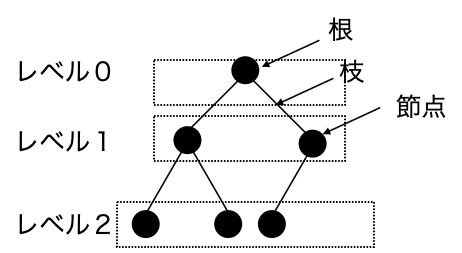
\includegraphics[width=100mm]{tree_example.png}
\end{center}
\end{figure}
この例ではレベルは2までとなります。

ヒープでは2分木を考え、特にデータの最大値を探しやすいようなデータ構造とします。のちに詳しく説明しますが、
ヒープでは最大値を根の位置に割り当てます。データを追加する際には追加したいデータと根を比較して大きな方を根に残します。
小さかった方は保持して左か右の子に移動して、同様のことを繰り返します。このとき、根から見て左右の木構造ができるだけバランスよく
構成されていた方が便利です。そこでヒープではデータ数が$n$のときは$k$
\begin{eqnarray}
2^{k}-1< n \leq 2^{k+1}-1
\end{eqnarray}
を満たす自然数として、レベル$k-1$までの全ての節点にデータを格納したのち、残りのデータをレベル$k$に格納することで木構造のバランスを保つようにします。
さらにレベル$k$にデータを追加するときも最も左の節点からデータを追加していきます。

このルールの下でヒープのかく節点に1から番号をつけていきます。まず根には1の番号を振ります。次にレベル1に移動し左から順に2、3の番号を振ります。
レベル2ではレベル1の2の節点の子の左から4、5を割り振り次にレベル1の3の節点の子の左から6、7の番号を振ります。以下同様に番号を振っていきます。
 \begin{figure}[H]
 \begin{center}
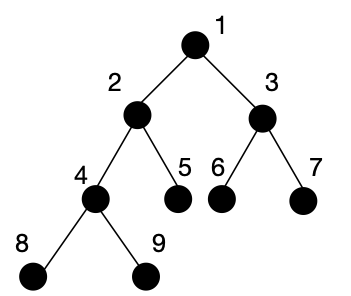
\includegraphics[width=100mm]{heap_number.png}
\end{center}
\end{figure}
今、一番大きなレベルの節点には左からデータを蓄えているので、このような番号づけで一意に節点を区別できます。またこの番号付だとm番目の節点の子の番号は
$2m$と$2m+1$で与えられることがわかります。
 \begin{figure}[H]
 \begin{center}
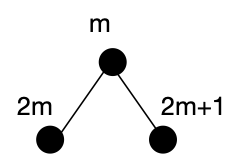
\includegraphics[width=100mm]{heap_number2.png}
\end{center}
\end{figure}
この番号付をプログラムの配列のラベルと同一視することで、配列を用いて木構造を表現することができます。

次に節点にデータを蓄える時のルールについて説明します。
ヒープではどの枝に対しても、親には子よりも大きなデータを保存するようにします。このルールにより根は必ずデータの最大値となります。
 \begin{figure}[H]
 \begin{center}
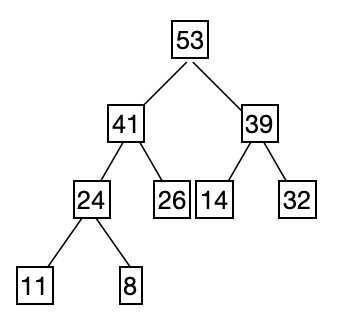
\includegraphics[width=100mm]{heap_store.png}
\end{center}
\end{figure}
ここまでの議論からデータ数がnのヒープの最大レベルは$[{\rm log}_{2}(n+1)]-1$で与えられることがわかります。
以上のルールをまとめます。
\begin{enumerate}
\item 根には番号1を割り当てます。
\item 番号$m$の左は$2m$で、右は$2m+1$とします。
\item データ数$n$を超える番号を持つ節点は存在しません。
\item どの枝に対しても、親は子よりも大きな数字を蓄えます。
\end{enumerate}

\subsubsection{ヒープへのデータの格納}
今n個のデータを蓄えているヒープがあるとして、そこに$n+1$個目のデータを追加する方法を考えます。まず、ヒープの木構造から$n+1$個目のデータを
追加したいときに増えるべき節点の位置は一意に決まります。$n+1$が偶数なら新たに追加する節点は$\frac{n+1}{2}$の左側の子、$n+1$が奇数なら新たに追加する節点は$\frac{n}{2}$の右側の子となります。
親の番号はどちらの場合もまとめて$[\frac{n+1}{2}]$となります。

$n+1$番目のデータの追加は次のように行います。以下では${\rm data}$という配列でヒープを表すことにます。
まず、追加したいデータを一時的に$n+1$番目の節点におきます。この時、追加した数字が親の数字より大きいときにはヒープのルールを満たしません。
そこで他との大小関係を確認する必要があります。親のデータは${\rm data}[[\frac{n+1}{2}]]$で与えられます。もし追加したデータが親のデータより大きい場合、すなわち
\begin{eqnarray}
{\rm data}[n+1]>{\rm data}[[\frac{n+1}{2}]]
\end{eqnarray}
の時には親のデータと交換します。交換したら、交換した先でさらに親のデータと大小関係を比較し親のデータが小さければ交換します。この作業を繰り返し子が親より小さなデータを蓄えるように
なったらデータの追加が完了です。以下に42の数字を追加するときのヒープの変化を示します。
 \begin{figure}[H]
 \begin{center}
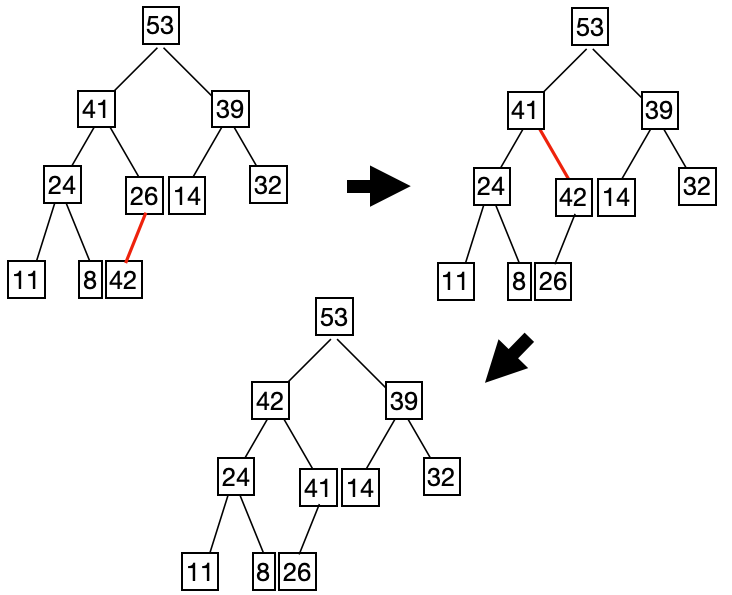
\includegraphics[width=100mm]{heap_append_example.png}
\end{center}
\end{figure}
赤色の線が子と親の代償関係が不整合になっている箇所です。そこの場所ではこのデータ(42)と親のデータ(26)を入れ替えます。入れ替えた先でさらに親のデータ(41)と追加データ(42)の大小関係が不整合
なのでデータを入れ替えます。最後には親と子の代償関係が整合するヒープが構成できました。

このヒープに対するデータの追加のアルゴリズムを疑似コード書くと以下のようになります。(配列のラベルは0から始めることに注意してください。)
\begin{figure}[H]
\begin{algorithm}[H]
	\caption{push heap}
	\label{push heap}
	\begin{algorithmic}[1]
	\STATE $x$ : 追加したいデータ 
	\STATE $n$: 追加する前のヒープが蓄えているデータ数
	\STATE $n ++$
	\STATE {\rm data}[n-1] = x
	\STATE $i=n$
	\STATE $j={\rm int}(i/2)$
	\WHILE{$j>0~\&~x > {\rm data}[j-1]$}
	\STATE {\rm data}[i-1]={\rm data}[j-1]
	\STATE $i=j$
	\STATE $j = {\rm int}(i/2)$
	\ENDWHILE
	\STATE ${\rm data}[i-1] = x$
	\end{algorithmic}
\end{algorithm}
\end{figure}
\subsubsection{最大データの取り出し}
次にヒープから最大の数を取り出す方法について説明します。
最大データは根にあります。問題は根のデータを削除した後に如何にしてヒープを再構成するのかです。
ヒープの根のデータを取り出すと、ヒープに蓄えられているデータの数が一つ減ります。ヒープを再構成するために、
まず一時的にヒープの末尾のデータを根に移動させます。これによってヒープの木構造は保たれます。しかし、末尾のデータは一般に小さな数字なので
それを根に移動すると親と子の大小関係が満たされなくなります。そこで親と子の大きさを比較してどちらかの子が親より大きかったら、データの移動が必要になります。
以下にヒープから最大値を取り出してヒープを再構成するアルゴリズムを示します。
\begin{figure}[H]
\begin{algorithm}[H]
	\caption{delete heap}
	\label{delete heap}
	\begin{algorithmic}[1]
	\STATE $n$: 削除する前のヒープが蓄えているデータ数
	\STATE $x={\rm data}[0]$
	\STATE $n--$
	\STATE ${\rm data}[0]={\rm data}[n-1]$
	\STATE $i=1$
	\WHILE{$2i \leq n$}
	\STATE $j=2i$
	\IF{$2i+1\leq n ~\&~{\rm data}[2i-1]<{\rm data}[2i]$}
	\STATE $j=2i+1$
	\ENDIF
	\IF{${\rm data}[i-1] \geq {\rm data}[j-1]$}
	\STATE break
	\ELSE
	\STATE $t={\rm data}[i-1]$
	\STATE ${\rm data}[i-1]={\rm data}[j-1]$
	\STATE ${\rm data}[j-1]=t$
	\ENDIF
	\STATE $i=j$
	\ENDWHILE
	\STATE return $x$
	\end{algorithmic}
\end{algorithm}
\end{figure}
\subsubsection{ヒープソート}
以上のヒープ構造を用いてソートを行うがヒープソートです。
ヒープソートでは最初にヒープにデータを追加するアルゴリズムを用いて、データを順に追加していきます。
全てのデータを追加した後に、順番に大きい数字から取り出していきます。
それでは実際に上で定義したpush\_heapとdelete\_heapを用いてソートをしてみます。
入力された配列は式(\ref{example init})で与えられるとして、順番にヒープに追加していきます。
最初は$5$を根に割り当てます。
\begin{eqnarray}
5, |N, N,| N, N, N, N,| N
\end{eqnarray}
今回はデータ数は8であることがわかっているので、配列のサイズを8で固定しておいて挿入されていない節点については$N$と表記してあります。
またレベルがわかりやすいようにレベルが変わる箇所で$|$を挿入しています。
次に$4$を追加すると
\begin{eqnarray}
5, |4, N,| N, N, N, N,| N
\end{eqnarray}
となります。次に追加するのは$8$です。先のアルゴリズムによるとまず一時的に$5$を蓄えている節点の右の子に$8$を置きます。
その後に親との大小関係を確認すると子($8$)の方が親($5$)よりも大きな数字なので親と子を入れ替えて、以下を得ます。
\begin{eqnarray}
5,| 4, 8,| N, N, N, N,| N\\
8,| 4, 5,| N, N, N, N,| N
\end{eqnarray}
$1,3,2$を追加しますが、こちらは親と子の大小関係は問題にならずに追加できます。
\begin{eqnarray}
8,| 4, 5,| 1, N, N, N,| N\\
8,| 4, 5,| 1, 3, N, N,| N\\
8,| 4, 5,| 1, 3, 2, N,| N
\end{eqnarray}
$7$の追加ではまず$5$を蓄えている節点の右の子に$7$を入れますが、親と子の大小関係を満たしてないので、
$5$と$7$を入れ替えます。
\begin{eqnarray}
8,| 4, 5,| 1, 3, 2, 7,| N\\
8,| 4, 7,| 1, 3, 2, 5,| N
\end{eqnarray}
最後に$6$を$1$の節点の左の子として追加しますが、親と子の大小関係を満たすように2回データの入れ替えを行います。
\begin{eqnarray}
8,| 4, 7,| 1, 3, 2, 5,| 6\\
8,| 4, 7,| 6, 3, 2, 5,| 1\\
8,| 6, 7,| 4, 3, 2, 5,| 1
\end{eqnarray}
これでヒープが完成します。以下にここまでの流れを図で示しています。赤色の枠が新しく追加した数字で、緑色の枠がデータ
が追加されたことで移動したデータとなります。
 \begin{figure}[H]
 \begin{center}
\includegraphics[width=100mm]{heap_example1.png}
\end{center}
\end{figure}
次に得られたヒープから最大のデータを順番に取り出していきます。
ヒープを配列で表現すると最大の数は必ず一番左になるのでまず、一番左のデータ(ヒープの根のデータ)を取り出します。
取り出すと根にデータがなくな理、ヒープ構造を保っていないので配列の末尾のダータを先頭に持っていき親と子の大小関係をみながらヒープを作成しなおします。
この操作を実際に見ていきます。いま先ほどのヒープがあるとします。
\begin{eqnarray}
8, |6, 7,| 4, 3, 2, 5,| 1
\end{eqnarray}
ここから$8$を取り出して末尾の$1$の数字を根に移動します。
すると根の部分で親と子の大小関係が崩れてしまうので、ヒープを保つためにデータを入れ替えます。
入れ替える時には左右の子のデータを比較して大きな数字を持つ子と親を入れ替えます。今回の場合には
根に$1$があり子の左が$6$で右が$7$なので、$7$と$1$を入れ替えます。すると今度は入れ替えた先で
親(1)と子(2,5)で大小関係を満たさないので$1$と$5$を入れ替えてヒープができました。
\begin{eqnarray}
1,| 6, 7,| 4, 3, 2, 5,| N\\
7,| 6, 1,| 4, 3, 2, 5,| N \\
7,| 6, 5,| 4, 3, 2, 1,| N 
\end{eqnarray}
次に$7$を取り出して再び末尾のデータの$1$を根に移動して、親子の大小関係を見ながらヒープを作り直していきます。
\begin{eqnarray}
1,| 6, 5,| 4, 3, 2, N,| N\\
6,| 1, 5,| 4, 3, 2, N,| N\\
6,| 4, 5,| 1, 3, 2, N,| N
\end{eqnarray}
以上同様に繰り返します。途中で作られるヒープだけ見ていくと以下のようは変遷をたどります。
\begin{eqnarray}
5, 4, 2, 1, 3, N, N, N\\
4, 3, 2, 1, N, N, N, N\\
3, 1, 2, N, N, N, N, N\\
2, 1, N, N, N, N, N, N\\
1, N, N, N, N, N, N, N
\end{eqnarray}
この最大値を順に取り出していく流れを以下に図に示します。
 \begin{figure}[H]
 \begin{center}
\includegraphics[width=100mm]{heap_example2.png}
\end{center}
\end{figure}
これらの手続きを疑似コードで書くと以下の通りです。
\begin{figure}[H]
\begin{algorithm}[H]
	\caption{heap sort}
	\label{heap sort}
	\begin{algorithmic}[1]
	\STATE ${\rm data}$: ソートしたい入力データ
	\STATE $n$:入力データの配列の長さ
	\FOR{$i=0;i<n;++i$}
	\STATE push\_heap(data[i])
	\ENDFOR
	\FOR{$i=0;i<n;++i$}
	\STATE data[n-i-1] = deleta\_heap()
	\ENDFOR
	\end{algorithmic}
\end{algorithm}
\end{figure}
ヒープは木構造の均衡が保たれているのでデータの追加と取り出しは$\mathcal{O}({\rm log}(n))$の計算量で済みます。故に全体としては$\mathcal{O}(n{\rm log}(n))$の
計算量で完了します。
\subsubsection{上記ヒープソートの改良}
ここまでのヒープソートでは入力データとは別にヒープを蓄える配列を一時的に用意してヒープソートを行ってきました。
しかし実はヒープではデータを蓄えていれる配列をそのままヒープとして扱うことができます。配列のk番目のデータを
ヒープに入れる時には、配列の0から$k-2$番目までをヒープとみなして操作をすることでそれを実現できます。
データを取り出すときも、取り出したデータを右から詰めていことで、配列をヒープとして扱うことができます。

またデータを順にヒープに追加してヒープを構成する方法についても改良することができます。
まず親子の大小関係を気にしないで与えられた配列が二分木を表しているとします。
親子関係を満たすように配列の末尾から親子関係を確認していきます。
配列の末尾から順番に接点を見ていき子を持つ節点を探します。この節点の子には配列の末尾のデータが含まれます。
もしその節点が子を一つ(末尾のデータ)しか持たないなら親と子の大小関係を比較して親が子よりも小さな数字の場合データを入れ替えます。
もし節点が子を二つ持つ場合には子のうち大きな数字を持つ方と親を比較して親の方が小さければ、二つを入れ替えます。この操作を配列の末尾から始めて子を持つ節点に対して行っていきます。
この操作を繰り返していくと、対象としている節点の子が子を持つようなケースも現れます。その場合にも、まず接点のデータと子のうち大きなデータを持つ子とを比較して、親の方が子よりも
小さな値の場合にはデータを入れ替えます。入れ替えた後に子と子の子と大小関係を比較し、必要があればデータを入れ替えます。以下この操作を大小関係が満たされるまで進めていきます。
以上の操作を繰り返すことで最終的にヒープ構造を作ることができます。この方法は、木構造の下の階層(高いレベル)から構造を見ていって部分木を整形してヒープを少しずつ作っていっています。

具体的にこの操作を式(\ref{example init})から始めてみていきます。
まず最初の配列を二分木とみなします。
\begin{eqnarray}
5, |4, 8, |1, 3, 2, 7,| 6
\end{eqnarray}
$|$は前回同様レベルが変わる箇所に挿入してあります。末尾から子を持つ節点を探します。ここでは$1$が格納されています。
(実際にはこの操作は配列の長さを$n$として${\rm int}(n/2)$番目の配列になります。)$1$が格納されている節点の子は$6$で親子の大小関係を満たしていないので$1$と$6$を入れ替えます。
\begin{eqnarray}
5,| 4, 8,| 6, 3, 2, 7,| 1
\end{eqnarray}
次に親になっている節点は$8$が格納されているますが、こちらの子(2と7)は親子の大小関係を満たしているので、そのままです。
次の親は$4$が格納されていますが、子(3,6)と大小関係を満たしていません。そこで子のうち大きな数字$6$と$4$を入れ替えます。入れ替えた後、子(新しく4が格納された節点)とその子をみてこちらは大小関係に問題ありません。
\begin{eqnarray}
5,| 6, 8,| 4, 3, 2, 7,| 1
\end{eqnarray}
次の親は根(5が格納)ですが子(6と8)と大小関係を満たしていないので、子のうち大きな数字(8)とデータを交換します。交換した先でも親(5)と子(2、7)が親子の大小関係を満たしていないのでデータ交換(5と7)を行って終了です。
\begin{eqnarray}
8, |6, 7,| 4, 3, 2, 5, |1
\end{eqnarray}
以上の操作を木構造を用いて表すと以下のようになります。
 \begin{figure}[H]
 \begin{center}
\includegraphics[width=100mm]{heap2_example1.png}
\end{center}
\end{figure}
緑色の節点と枝が整形が完了した箇所になります。改良されたヒープソートのアルゴリズムの疑似コードを以下にまとめます。
\begin{figure}[H]
\begin{algorithm}[H]
	\caption{heap sort 2}
	\label{heap sort 2}
	\begin{algorithmic}[1]
	\STATE ${\rm data}$: ソートしたい入力データ
	\STATE $n$:入力データの配列の長さ
	\FOR{$k={\rm int}(n/2);k>0;--k$}
	\STATE $i=k$
	\STATE $j=2i$
	\STATE $x = {\rm data}[i-1]$
	\WHILE{$j\leq n$}
	\IF{$j<n \& {\rm data}[j] > {\rm data}[j-1]$}
	\STATE $j=j+1$
	\ENDIF
	\IF{$x<{\rm data}[j-1]$}
	\STATE ${\rm data}[i-1] = {\rm data}[j-1]$
	\STATE $i=j$
	\STATE $j=2i$
	\ELSE
	\STATE break
	\ENDIF
	\ENDWHILE
	\STATE ${\rm data}[i-1]=x$
	\ENDFOR
	\FOR{$k=n-1;0<k-1;--k$}
	\STATE $x={\rm data}[k]$
	\STATE ${\rm data}[k] = {\rm data}[0]$
	\STATE $i=1$
	\STATE $j=2$
	\WHILE{$j\leq k$}
	\IF{$j<k \& {\rm data}[j] > {\rm data}[j-1]$}
	\STATE $j = j +1$
	\ENDIF
	\IF{$x<{\rm data}[j-1]$}
	\STATE ${\rm data}[i-1] = {\rm data}[j-1]$
	\STATE $i=j$
	\STATE $j=2i$
	\ELSE
	\STATE break
	\ENDIF
	\ENDWHILE
	\STATE ${\rm data}[i-1]=x$
	\ENDFOR
	\end{algorithmic}
\end{algorithm}
\end{figure}
この疑似コードでは、3行目のループでヒープを作成し21行目でデータを取り出しています。
このアルゴリズムではヒープを作成する箇所の計算量を推定します。簡単のため$n=2^{k}-1$をデータ数とします。
この時レベル$k$が最高レベルとなります。レベル$j(\leq k)$における節点を根とした部分木を作るためには
部分木の高さが$k-j$なのでデータの比較としてはたかだか$2(k-j)$程度です。レベル$j$除ける接点の数は$2^{j-1}$なので計算量としては
\begin{eqnarray}
\sum_{j=1}^{k-1}2(k-j)2^{j-1}=2^{k+1}-2k-2<2n
\end{eqnarray}
となり$\mathcal{O}(n)$以下に抑えられることがわかります。
\subsection{クイックソート}
クイックソートは
\begin{thebibliography}{9}
\item 辻真吾、下平英寿、「Pythonで学ぶアルゴリズムとデータ構造」
\end{thebibliography}

\end{document}
